% Presentation to WNAR in Honolulu, June 2014


\documentclass{beamer}
\usepackage[T1]{fontenc}
\usepackage{graphicx}
\usetheme{Warsaw}

%%%%%%%%%%%%%%%%%%%%%%%%%%%%%%%%%%%%%%%command added by me
\usepackage{array}
\usepackage{tabularx}
\usepackage{multirow} 
\usepackage{multirow}
%\usepackage{subfig}


% refer to the following URL for hints on beamer
%        http://www.math.umbc.edu/~rouben/beamer/quickstart-Z-H-27.html#node_sec_27
%gets rid of bottom navigation bars
\setbeamertemplate{footline}[page number]{}

%gets rid of navigation symbols
\setbeamertemplate{navigation symbols}{}

% set background color to light shade of blue
\setbeamercolor{normal text}{bg=blue!12}

% To create 2 x3 handouts
% use the Preview program in Macintosh. You can set up the number of slides/page with the layout options
% in the usual fashion.
% Note that Adobe will not let you save a pdf file to another pdf file using the print -> pdf options - you must use Preview
\usepackage{fancyvrb}
\usepackage{relsize}





%\usecolortheme{beaver}
%%%%%%%%%%%%%%%%%%%%%%%%%%%%%%%%%%%%%%%%%%%%%%%%%%%%%%%%%%%%%%%%%%%%%
%\beamersetuncovermixins{\opaqueness<1>{25}}{\opaqueness<2->{15}}

\title[WNAR 2014]{Partial Stratification in Two-Sample Capture-Recapture Experiments}  
\author[Lasantha Premarathna]{Lasantha Premarathna\\Carl James Schwarz}
\institute[SFU]{Department of Statistics and Actuarial Science, \\ Simon Fraser University, \\ Burnaby, BC.}
\date{\today}


\begin{document}

%%%%%%%%%%%%%%%%%%%%%%%%%%%%%%%%%%%%%%%%%%%%%%%%%%%%%%%%%%%%%%%%%%%%%%%%%%%%%%%%%%%%
\begin{frame}
\titlepage
\end{frame}
%%%%%%%%%%%%%%%%%%%%%%%%%%%%%%%%%%%%%%%%%%%%%%%%%%%%%%%%%%%%%%%%%%%%%%%%%%%%%%%%%%%%
\begin{frame}\frametitle{Basic capture-recapture}
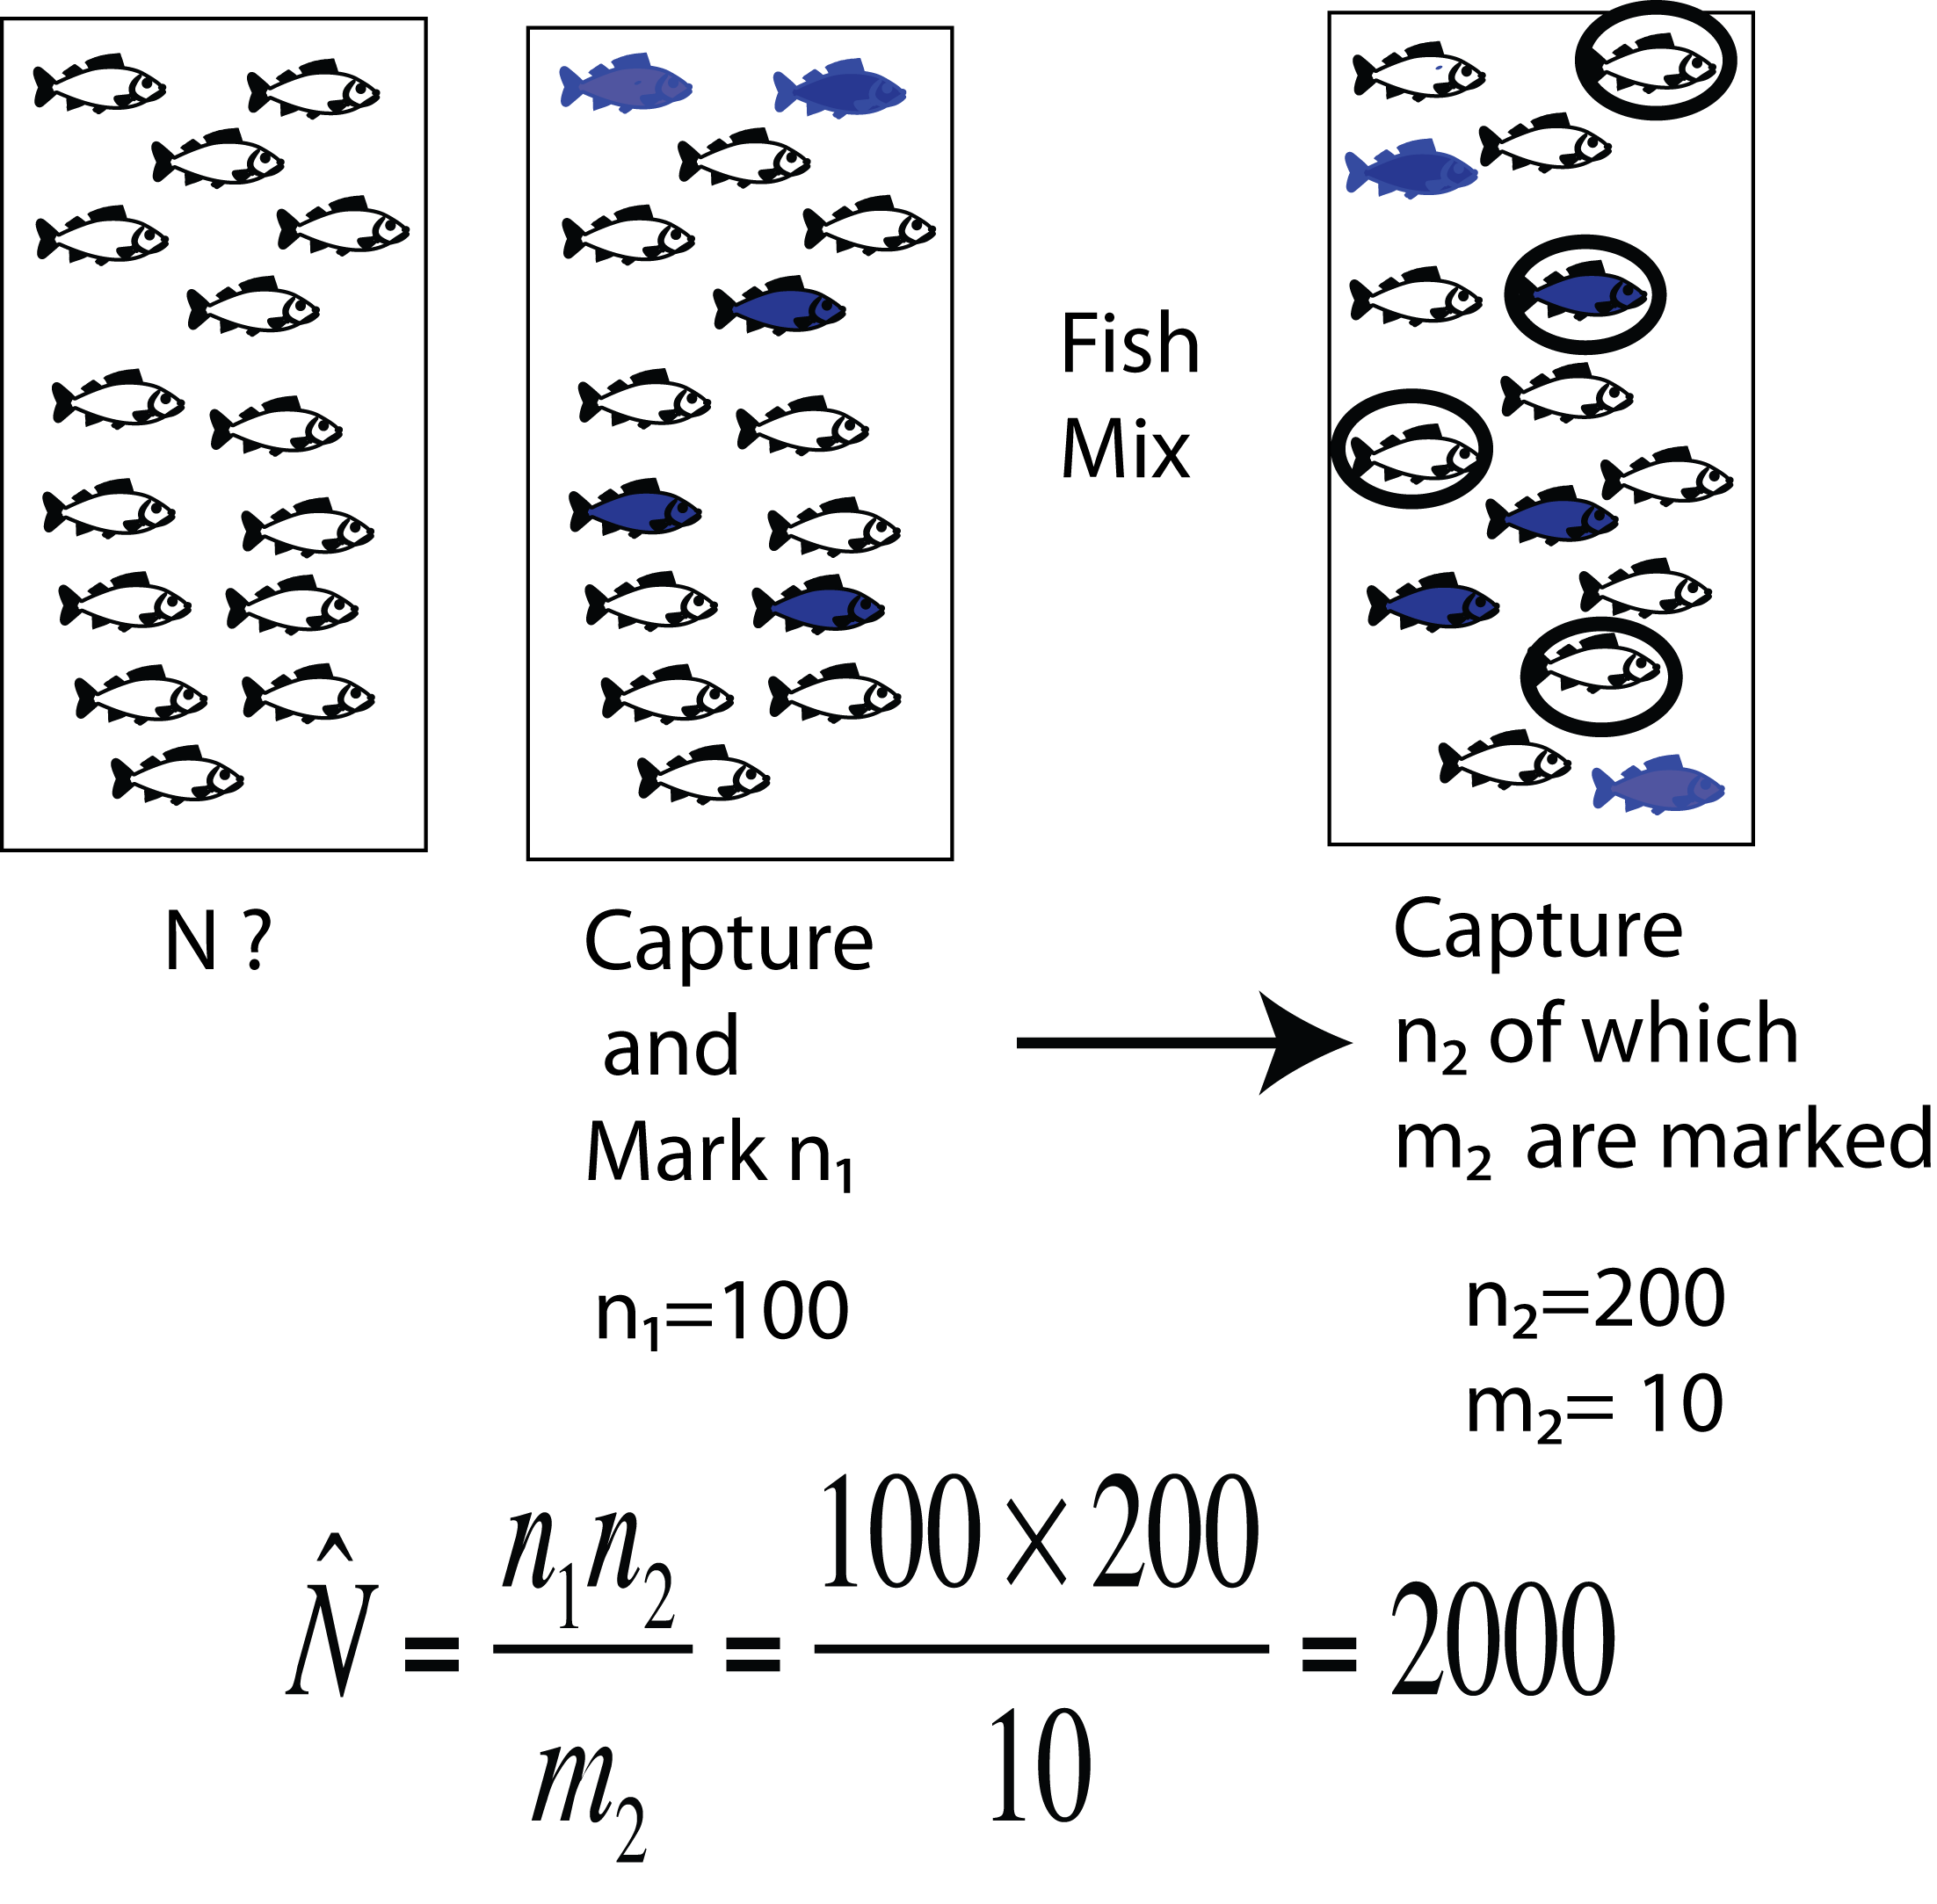
\includegraphics[height=0.90 \textheight]{PetersenIntro}
\end{frame} 


%%%%%%%%%%%%%%%%%%%%%%%%%%%%%%%%%%%%%%%%%%%%%%%%%%%%%%%%%%%%%%%%%%%%%%%%%%%%%%%%%%%%
\begin{frame}\frametitle{Standard Lincoln-Petersen - Assumptions}

\begin{itemize}
 \item The population is \textbf{closed} (geographically and demographically). 
 \item Mark status is correctly identified at each sampling occasion
 \item Marks are not lost between sampling occasions
 \item Capture and marking does not affect subsequent catchability of an animal
 \item Sampling is random
 \item {\bf Homogeneous capture probabilities.}
 \end{itemize}
 $$\widehat{N} = \frac{n_1 \times n_2}{m_2} \approx \frac{ Np_1 \times Np_2}{Np_1p_2} \approx N$$
 
\end{frame}

%%%%%%%%%%%%%%%%%%%%%%%%%%%%%%%%%%%%%%%%%%%%%%%%%%%%%%%%%%%%%%%%%%%%%%%%%%%%%%%%%%%%
\begin{frame}\frametitle{Standard Lincoln-Petersen - Need for stratification}
Animals may vary in catchability, e.g.\ by sex.\\
This can lead to biases when heterogeneity is ignored.\\[5mm]

\begin{tabular}{lrrr | rrr | r}
Sex & $N$ &  $p_1$ & $p_2$ &   $n_1$ & $n_2$ & $m_2$ & $\widehat{N}$ \\ \hline
M &  1200 & .10  & .05 &   120 &  60  &  6    \\
F  &    800 & .05  & .10 &     40 &  80  &  4     \\ \hline
Total & 2000 &     &       &   160 & 140 & 10 & 2240 \\ \hline
\end{tabular}

\vspace{3mm}
Bias can go in either direction depending on correlation of catchabilities.

 
\end{frame}


\begin{frame}\frametitle{Standard Lincoln-Petersen - Need for stratification}
Animals may vary in catchability, e.g.\ by sex. \\[2mm]
{\bf Stratify and compute separate estimates for each stratum.}\\[5mm]

\begin{tabular}{lrrr | rrr | r}
Sex & $N$ &  $p_1$ & $p_2$ &   $n_1$ & $n_2$ & $m_2$ & $\widehat{N}$ \\ \hline
M &  1200 & .10  & .05 &   120 &  60  &  6  &   1200\\
F  &    800 & .05  & .10 &     40 &  80  &  4  & 800   \\ \hline
Total & 2000 &     &       &    &  &  & 2000 \\ \hline
\end{tabular}

\vspace{3mm}
{\bf Assumes that you can classify animals into strata in ALL sampling occasions.}

 
\end{frame}



\begin{frame}\frametitle{Partial Stratification} %\[allowframebreaks]{Introduction} 
Sometimes difficult/costly to stratify when captured.\\
Select a sub-sample of each sample to stratify.

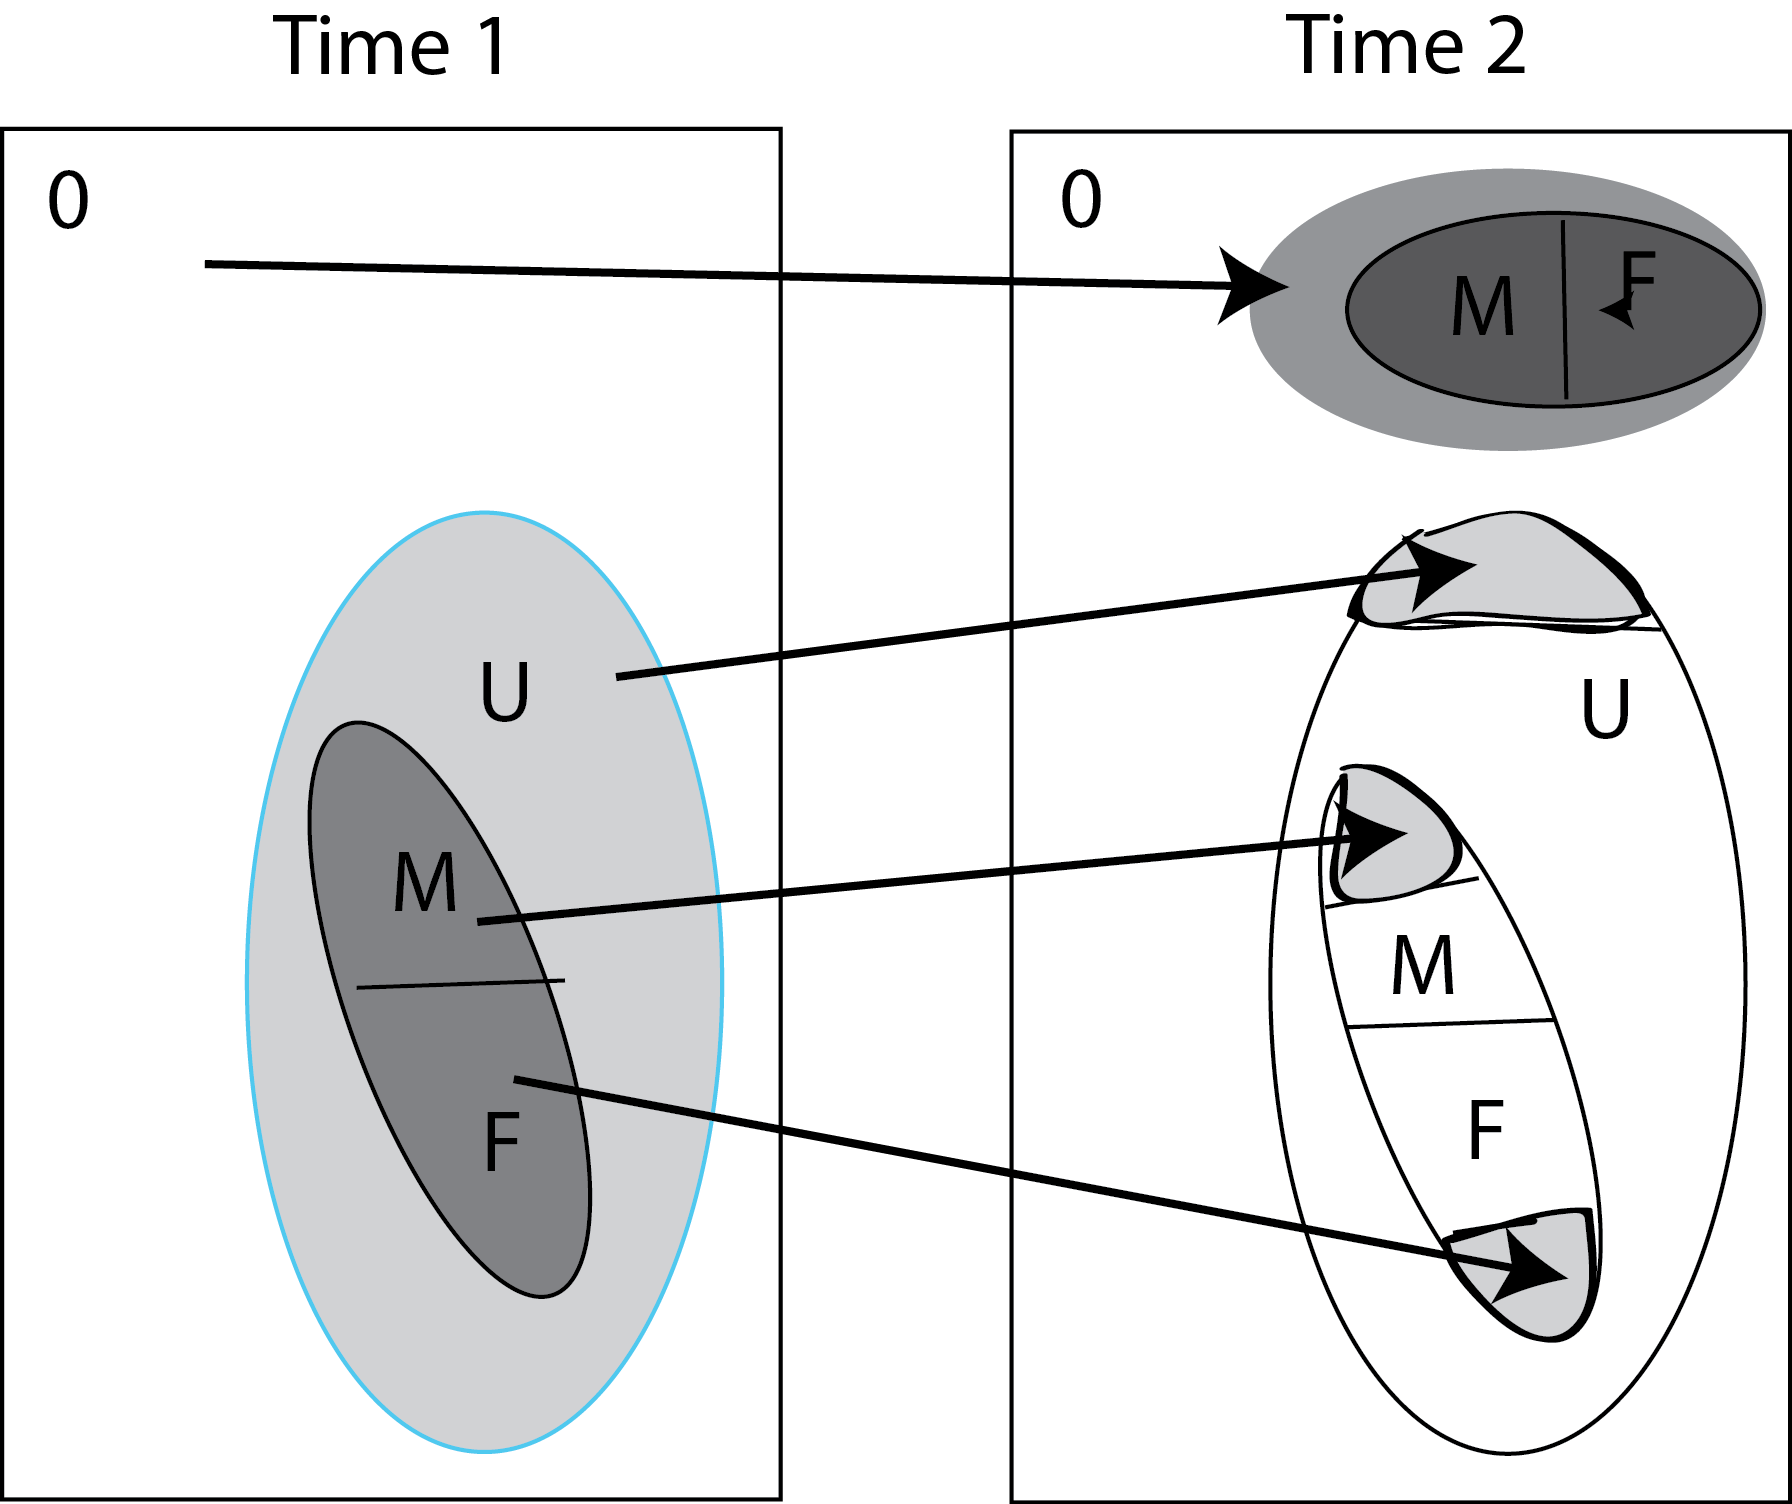
\includegraphics[height=0.8 \textheight]{PartialStrat.png}

\end{frame}


%%%%%%%%%%%%%%%%%%%%%%%%%%%%%%%%%%%%%%%%%%%%%%%%%%%%%%%%%%%%%%%%%%%%%%%%%%%%%%%%

\begin{frame} \frametitle{Partial Stratification}

$3C + 4$ possible capture histories.\\[2mm]

\begin{tabular}{ll} \hline
History & Probability \\ \hline
MM     &  $\lambda_{M}\  p_{1M} \ \theta_1 \ p_{2M}$ \\ 
M0      &  $\lambda_{M} \ p_{1M} \ \theta_1 \ (1-p_{2M})$ \\
0M      &  $\lambda_{M} \ (1-p_{1M})\ p_{2M}\ \theta_{2} $\\
$\ldots$ & Similarly for other categories \\
\\
UU      &  $\lambda_{M} \ p_{1M}\ (1-\theta_1)\ p_{2M} + \lambda_{F} \ p_{1F} \ (1-\theta_1) \ p_{2F}$ \\
U0      &  $\lambda_{M} \ p_{1M}\ (1-\theta_1)\ (1-p_{2M}) + \lambda_{F} \ p_{1F} \ (1-\theta_1) \ (1-p_{2F})$ \\
0U      &  $\lambda_{M} \ (1-p_{1M}) \ p_{2M} \ (1-\theta_2) + \lambda_{F} \ (1-p_{1F}) \ p_{2F} \ (1-\theta_2)$ \\
 \\
00   &  Everything else (not observable) \\ \hline
\end{tabular}
Where
\begin{itemize}
\item $p_{tC}$ = probability of capture at time $t$ of category $C$.
\item $\lambda_C$ = proportion of category $C$ in the population.
\item $\theta_t$ = proportion of sample at time $t$ that is ``categorized''.
\end{itemize} 
\end{frame}


%%%%%%%%%%%%%%%%%%%%%%%%%%%%%%%%%%%%%%%%%%%%%%%%%%%%%%%%%%%%%%%%%%%%%%%%%%%%%%%%

%\subsection{Likelihood}
\begin{frame} \frametitle{Partial Stratification - Likelihood }

Multinomial distribution with unknown index\\
\vspace{6pt}

 \begin{multline*}
% \begin{split}
L = \frac{N!}{n_{U0}!\quad n_{UU}!\quad n_{0U}! \ldots \quad (N-n)!} \quad \times \\
 (P_{U0})^{n_{U0}}(P_{UU})^{n_{UU}}(P_{0U})^{n_{0U}} \quad \times \\
\prod_{C} (P_{C0})^{n_{C0}} \  \times \quad
 \prod_{C} (P_{CC})^{n_{ CC}} \quad \times
\quad \prod_{C} (P_{0C})^{n_{0C}} \quad \times \quad (P_{00})^{N-n}\\
%\end{split}
 \end{multline*}
\end{frame}


%%%%%%%%%%%%%%%%%%%%%%%%%%%%%%%%%%%%%%%%%%%%%%%%%%%%%%%%%%%%%%%%%%%%%%%%%%%%%%%%%%%%%%
%%%%%%%%%%%%%%%%%%%%%%%%%%%%%%%%%%%%%%%%%%%%%%%%%%%%%%%%%%%%%%%%%%%%%%%%%%%%%%%%%%%%%%
%\subsection{Parameter Estimation}
\begin{frame} \frametitle{Partial Stratification -  Estimation}

No closed form solution - standard numerical methods used. \\[5mm]

Parameters can be constrained by using the design matrix  and offset vectors 
$$ logit(p_{tk}) = X \beta + offset$$

Example, a model with  $p_{1M} = p_{1F}$ ,  $p_{2M} = p_{2F}$
uses design matrices and offsets\\
\begin{center} logit(
$\begin{bmatrix}
p_{1M}\\
p_{1F}\\
p_{2M}\\
p_{2F}\\
\end{bmatrix}$ )=
$\begin{bmatrix}
1 & 0\\
1 & 0\\
0 & 1 \\
0 & 1 \\
 \end{bmatrix}$ 
$\begin{bmatrix}
\beta_{1}\\
\beta_{2}\\
\end{bmatrix}$
 + 
$ \begin{bmatrix}
0\\
0\\
0\\
0\\
\end{bmatrix}$
\end{center}

\end{frame}


%The PIM is just a convenient method to describe the design matrix. GIve the general case here, i.e logit(parm) = X beta + Offset and then give examples of equal capture probs for m & f, and for fixed values of parameters such as the sex 

%%%%%%%%%%%%%%%%%%%%%%%%%%%%%%%%%%%%%%%%%%%%%%%%%%%%%%%%%%%%%%%%%%%%%%%%%%%%%%%%%%%%%%
%%%%%%%%%%%%%%%%%%%%%%%%%%%%%%%%%%%%%%%%%%%%%%%%%%%%%%%%%%%%%%%%%%%%%%%%%%%%%%%%%%%%%%
%\section{Model Selection}
\begin{frame} \frametitle{Partial Stratification - Model Selection}
Use Akaike's information criterion ($AIC$) ( Burnham and Anderson, 2002) to rank models.\\[2mm]
\end{frame}


\begin{frame}\frametitle{Partial Stratification - Optimal Allocation}

Use linear cost function
$$
C = n_{1} c_{1}  + n_{1}^{*} c_{1}^{*} +  n_{2} c_{2}  + n_{2}^{*} c_{2}^{*} \leq C_{0}
$$
where
\begin{itemize}
\item $n_1$ is number of fish captured at first occasion;
\item $n_1^*$ is number of fish captured at first occasion that are ``categorized''. $n_1 \geq n_1^*$.
\item $n_2$ is the number  of fish captured at second occasion;
\item $n_2^*$ is the number of fish captured at second occasion that are ``categorized''. $n_2 \geq n_2^*$.
\end{itemize}

\end{frame}

%%%%%%%%%%%%%%%%%%%%%%%%%%%%%%%%%%%%%%%%%%%%%%%%%%%%%%%%%%%%%%%%%%%%%%%%%%%%%%%%%%%%%%
%%%%%%%%%%%%%%%%%%%%%%%%%%%%%%%%%%%%%%%%%%%%%%%%%%%%%%%%%%%%%%%%%%%%%%%%%%%%%%%%%%%%%%
%\section{Example}
\begin{frame} \frametitle{Partial Stratification - Example}
\textbf{Walleye Data-Mille Lacs, MN} 
\vspace{3pt}

\begin{itemize}
\item Walleye are captured on the spawning grounds. Almost all the fish can be sexed in the first occasion
\item All the captured fish are tagged and released and the recapture occurred 3 weeks later using gill-nets
\item From a sample of fish captured at second occasion that are not tagged, a random sample is selected and sexed
\end{itemize} 

\begin{center}
\begin{tabular}{ |l|r| } 
\hline
  Capture History & statistics \\ \hline
  $U0$ & 40 \\ \hline
  $UU$ & 1 \\ \hline
  $M0$ & 5067 \\ \hline
  $MM$ & 40 \\ \hline
  $F0$ & 1551 \\ \hline
  $FF$ & 33 \\ \hline
  $0M$ & 41 \\ \hline
  $0F$ & 237 \\ \hline
  $0U$ & 3075 \\ \hline
\end{tabular}
\end{center}




\end{frame}


%%%%%%%%%%%%%%%%%%%%%%%%%%%%%%%%%%%%%%%%%%%%%%%%%%%%%%%%%%%%%%%%%%%%%%%%%%%%%%%%%%%%%%

\begin{frame} \frametitle{Partial Stratification - Example}
\vspace{3pt}

\begin{tabular}{lllrrrrrr}\hline 
\multicolumn{3}{c}{Model}                        & np  &$\hat{N}$  &$s.e.(\hat{N}$) &$\Delta AICc$ \\
                 &                   &                        &        &         '000s       & '000s & \\  \hline
 $p(C*t)$  & $\theta(t)$ & $\lambda(C) $  & 8    &      205  & 26     &        0.0\\ 
$p(C*t)$   & $\theta(t)$ & $\lambda(.)$     & 7    &      208  & 24    &        4.7\\ 
$p(t)$       & $\theta(t)$ & $\lambda(C)$     & 6     &     311   & 36   &    462.2 \\
$p(C)$     & $\theta(t)$ &  $\lambda(C)$   & 6    &      399  & 54    &   1561.5\\ 
 $p(.)$      & $\theta(t)$ & $\lambda(C)$   & 5    &      348  & 39    &   1572.0\\ 
 $p(C)$     & $\theta(t)$ & $\lambda(.)$     & 5    &     399  & 54    &  11613.4\\
 $p(.)$      & $\theta(.)$ & $\lambda(.)$     & 3    &     348  & 39    &  13276.8\\ \hline
 \end{tabular}\\
\begin{itemize}
\item $p$ = probability of capture 
\item $\lambda$ = proportion of category in the population.
\item $\theta$ = proportion of sample at time that is ``categorized''.
\item $C*t$ = varies by category and time; 
\item $t$ = varies by time but not category;
\item $C$ = varies by category but not by time
\item $.$ = no variation by time or by category.
\end{itemize} 
\end{frame}

%%%%%%%%%%%%%%%%%%%%%%%%%%%%%%%%%%%%%%%%%%%%%%%%%%%%%%%%%%%%%%%%%%%%%%%%%%%%%%%%%%%%%%
\begin{frame} \frametitle{Partial Stratification - Example}
\begin{tabular}{lrrr}
\hline
Parameter        & MLE       & SE     &  SE  if sex ratio known \\ \hline
$\lambda_{M}$ & .33     & .06   &   - \\ 
$\lambda_{F}$  & .67     & .06   &  - \\ \hline
\\ 
$\theta_{1}$     & .993     & .001  &  .001 \\ 
$\theta_{2}$     & .082    &  .004  &  .004 \\ \hline
\\
$N$         & 205,000     	 &   26,000   &  25,000    \\ \hline
$N_{M}$ &  68,000     	 &   13,000     &   8,000  \\ 
$N_{F}$ & 137,000          &   23,000    &  17,000    \\ \hline \hline
\\
$\hat{N}_{LP}$ & 311,000   & 36,000  & \\ \hline

\end{tabular}


\end{frame}


%%%%%%%%%%%%%%%%%%%%%%%%%%%%%%%%%%%%%%%%%%%%%%%%%%%%%%%%%%%%%%%%%%%%%%%%%%%%%%%%%%%%%%
%%%%%%%%%%%%%%%%%%%%%%%%%%%%%%%%%%%%%%%%%%%%%%%%%%%%%%%%%%%%%%%%%%%%%%%%%%%%%%%%%%%%%%
\begin{frame} \frametitle{Example - optimal allocation}
Let $c_{1} =2 $, $c_{2} =c_{1}/2$, $c_{1}^{*} = 4$, $c_{2}^{*} = c_{1}^{*}/2 = 4$, $C_{0} =40000$\\[5mm]

 Optimal $n_{1} = 8199 $ \  $n_{1}^{*} = 3003$  \  $n_{2} = 9511$ \  $n_{2}^{*} = 997$ \\
 leading to $SE(\widehat{N}) = 16000$ a 30\% reduction.\\[2mm]
 
Contour plot for $SE(\widehat{N})$ with $x$ current allocation and $o$ optimal allocation.\\
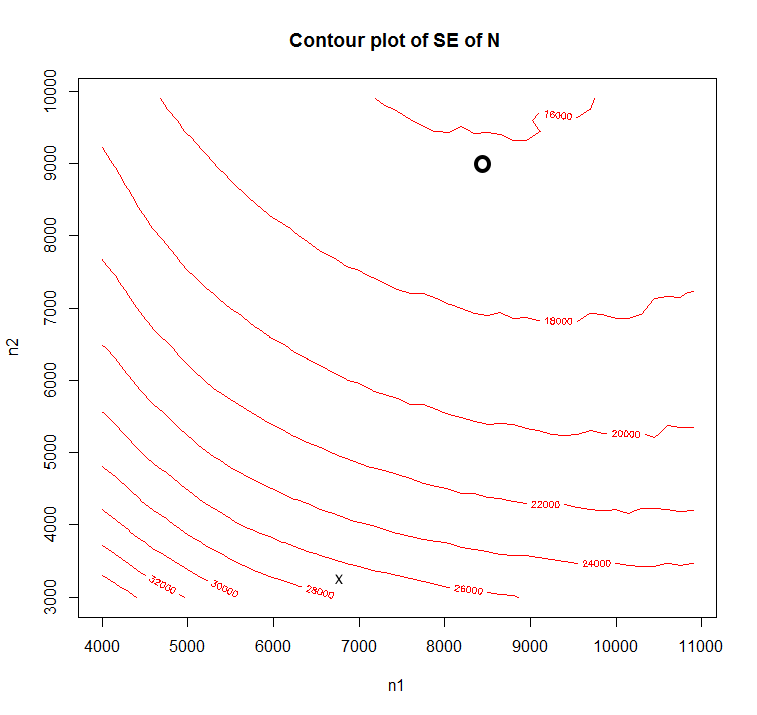
\includegraphics[scale=.20]{2014_05_19Contour_plot.png}

\end{frame}

%%%%%%%%%%%%%%%%%%%%%%%%%%%%%%%%%%%%%%%%%%%%%%%%%%%%%%%%%%%%%%%%%%%%%%%%%%%%%%%
\begin{frame} \frametitle{Partial Stratification - Summary}

Problem
\begin{itemize}
\item Capture heterogeneity can cause bias in estimates in capture-recapture experiments 
\item Stratification may not be possible/is costly for all captured animals in each occasion
\end{itemize}

Solution
\begin{itemize}
\item Partial stratification 
\item Optimal allocation 
\end{itemize}

Future work
\begin{itemize}
\item Bayesian solution for prior information on sex ratio
\item Individual covariates such as length
\end{itemize}
\end{frame}


\end{document}